\documentclass[11pt,a4paper]{article}
\usepackage[margin=2.4cm,top=2.2cm]{geometry}
\usepackage{amsmath,amssymb}
\usepackage{tgschola}\usepackage{fouriernc}
\linespread{1.05}
\usepackage[T1]{fontenc}
\usepackage{microtype}
\usepackage{tikz}
\usetikzlibrary{angles,quotes,calc,arrows.meta}
\usepackage{enumitem}
\usepackage{needspace}
\usepackage{tfrupee}
\definecolor{figline}{RGB}{64,64,64}
\definecolor{figfill}{RGB}{232,232,232}
\definecolor{figfill2}{RGB}{214,214,214}
\definecolor{muted}{RGB}{72,74,78}
\definecolor{thinrule}{RGB}{128,128,128}
\pagestyle{plain}
\setlength{\parindent}{0pt}
\setlength{\parskip}{1pt}
\setlength{\lineskiplimit}{2pt}\setlength{\lineskip}{4pt}
\setlength{\emergencystretch}{2em}
\tikzset{fig/.style={draw=figline}}
\newcommand{\nl}{\\[3pt]}
\newcounter{qn}
\newcommand{\ques}{\par\medskip\refstepcounter{qn}\noindent\hangindent=1.7em\hangafter=1\makebox[1.7em][l]{\textbf{\arabic{qn}.}}\ignorespaces}
\newcommand{\pc}[2]{\par\smallskip\noindent\hspace*{2em}\hangindent=4.3em\hangafter=1\makebox[2em][l]{(#1)}\hspace{0.3em}#2\par}
\newcommand{\mcqone}[4]{\par\smallskip\noindent\hspace*{2em}\hangindent=4.3em\hangafter=1(a)~#1 \qquad (b)~#2 \qquad (c)~#3 \qquad (d)~#4\par}
\newcommand{\mcqtwo}[4]{\par\smallskip\noindent\hspace*{2em}\begin{tabular}[t]{@{}p{0.42\linewidth}@{\hspace{1.6em}}p{0.42\linewidth}@{}}(a)~#1 & (b)~#2 \\[5pt](c)~#3 & (d)~#4\end{tabular}\par\smallskip}
\newcommand{\optline}[1]{\par\vspace{2pt}\noindent\hspace*{2em}\hangindent=4.3em\hangafter=1 #1}
\newcommand{\aritem}[2]{\par\smallskip\noindent\hspace*{1.7em}\hangindent=1.7em\hangafter=1 #1:~#2\par}
\newcommand{\orline}{\par\smallskip{\centering\textit{OR}\par}\nopagebreak\smallskip}
\newcommand{\sect}[1]{\par\medskip\Needspace{15\baselineskip}{\small\bfseries #1}\par\nopagebreak\smallskip}
\ifteacher
\newenvironment{answerblock}
  {\par\needspace{6\baselineskip}\smallskip\begingroup\small\linespread{1.2}\selectfont\color{muted}\noindent\textit{Answer.}\par}
  {\par\endgroup\medskip}
\newcommand{\ap}[1]{\par\smallskip\noindent\textbf{(#1)}\ }
\else
\usepackage{comment}
\excludecomment{answerblock}
\fi
\makeatletter
\newcommand{\figslot}[1]{\@ifundefined{fig@#1}{}{\csname fig@#1\endcsname}}
\makeatother
\makeatletter\expandafter\def\csname fig@a1\endcsname{%
\begin{center}
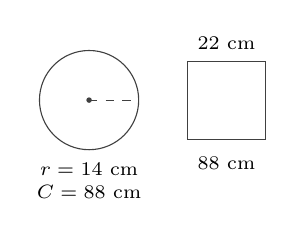
\begin{tikzpicture}[fig,every node/.style={font=\scriptsize}]
\draw[fig] (0,0) circle (0.63);
\fill[figline] (0,0) circle (0.035);
\draw[fig,dashed] (0,0) -- (0.63,0);
\node[below,align=center] at (0,-0.68) {$r=14$~cm\\$C=88$~cm};
\draw[fig] (1.25,-0.495) rectangle (2.24,0.495);
\node[above] at (1.745,0.52) {$22$~cm};
\node[below] at (1.745,-0.6) {$88$~cm};
\end{tikzpicture}
\end{center}}

\expandafter\def\csname fig@a2\endcsname{%
\begin{center}
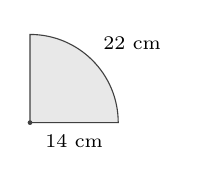
\begin{tikzpicture}[fig,every node/.style={font=\scriptsize}]
\fill[figfill] (0,0) -- (1.12,0) arc (0:90:1.12) -- cycle;
\draw[fig] (0,0) -- (1.12,0) arc (0:90:1.12) -- cycle;
\fill[figline] (0,0) circle (0.03);
\node[below] at (0.56,-0.03) {$14$~cm};
\node[above right] at (45:1.14) {$22$~cm};
\end{tikzpicture}
\end{center}}

\expandafter\def\csname fig@a3\endcsname{%
\begin{center}
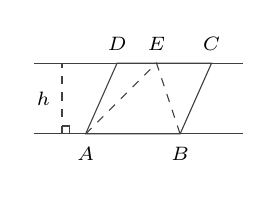
\begin{tikzpicture}[fig,every node/.style={font=\scriptsize}]
\draw[fig,thin] (-0.35,0) -- (2.3,0);
\draw[fig,thin] (-0.35,0.9) -- (2.3,0.9);
\draw[fig] (0.3,0) -- (0.7,0.9) -- (1.9,0.9) -- (1.5,0) -- cycle;
\draw[fig,dashed] (0.3,0) -- (1.2,0.9) -- (1.5,0);
\draw[fig,dashed] (0,0) -- (0,0.9);
\draw[fig] (0,0.1) -- (0.1,0.1) -- (0.1,0);
\node[left] at (-0.03,0.45) {$h$};
\node[below] at (0.3,-0.04) {$A$};
\node[below] at (1.5,-0.04) {$B$};
\node[above] at (0.7,0.94) {$D$};
\node[above] at (1.9,0.94) {$C$};
\node[above] at (1.2,0.94) {$E$};
\end{tikzpicture}
\end{center}}

\expandafter\def\csname fig@a4\endcsname{%
\begin{center}
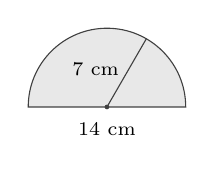
\begin{tikzpicture}[fig,every node/.style={font=\scriptsize}]
\fill[figfill] (-1,0) arc (180:0:1) -- cycle;
\draw[fig] (-1,0) arc (180:0:1) -- cycle;
\fill[figline] (0,0) circle (0.03);
\draw[fig] (0,0) -- (60:1);
\node[left] at (60:0.55) {$7$~cm};
\node[below] at (0,-0.08) {$14$~cm};
\end{tikzpicture}
\end{center}}

\expandafter\def\csname fig@a5\endcsname{%
\begin{center}
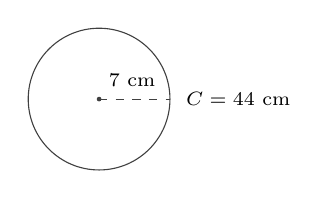
\begin{tikzpicture}[fig,every node/.style={font=\scriptsize}]
\draw[fig] (0,0) circle (0.9);
\fill[figline] (0,0) circle (0.03);
\draw[fig,dashed] (0,0) -- (0.9,0);
\node[above] at (0.42,0.03) {$7$~cm};
\node[right] at (0.98,0) {$C=44$~cm};
\end{tikzpicture}
\end{center}}

\expandafter\def\csname fig@a6\endcsname{%
\begin{center}
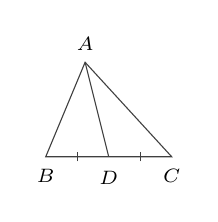
\begin{tikzpicture}[fig,every node/.style={font=\scriptsize}]
\draw[fig] (0,0) -- (1.6,0) -- (0.5,1.2) -- cycle;
\draw[fig] (0.5,1.2) -- (0.8,0);
\draw[fig] (0.4,-0.06) -- (0.4,0.06);
\draw[fig] (1.2,-0.06) -- (1.2,0.06);
\node[above] at (0.5,1.23) {$A$};
\node[below] at (0,-0.04) {$B$};
\node[below] at (1.6,-0.04) {$C$};
\node[below] at (0.8,-0.06) {$D$};
\end{tikzpicture}
\end{center}}

\expandafter\def\csname fig@b7\endcsname{%
\begin{center}
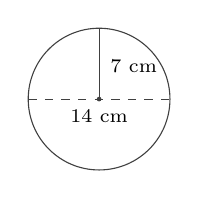
\begin{tikzpicture}[fig,every node/.style={font=\scriptsize}]
\draw[fig] (0,0) circle (0.9);
\fill[figline] (0,0) circle (0.03);
\draw[fig,dashed] (-0.9,0) -- (0.9,0);
\draw[fig] (0,0) -- (0,0.9);
\node[right] at (0.02,0.42) {$7$~cm};
\node[below] at (0,-0.02) {$14$~cm};
\end{tikzpicture}
\end{center}}

\expandafter\def\csname fig@b8\endcsname{%
\begin{center}
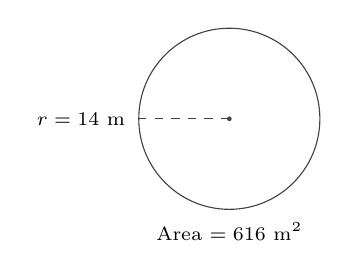
\begin{tikzpicture}[fig,every node/.style={font=\scriptsize}]
\draw[fig] (0,0) circle (1.15);
\fill[figline] (0,0) circle (0.03);
\draw[fig,dashed] (0,0) -- (-1.15,0);
\node[left] at (-1.2,0) {$r=14$~m};
\node[below] at (0,-1.2) {Area $=616$~m$^2$};
\end{tikzpicture}
\end{center}}

\expandafter\def\csname fig@b9\endcsname{%
\begin{center}
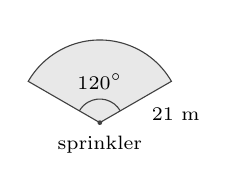
\begin{tikzpicture}[fig,every node/.style={font=\scriptsize}]
\fill[figfill] (0,0) -- (30:1.05) arc (30:150:1.05) -- cycle;
\draw[fig] (0,0) -- (30:1.05) arc (30:150:1.05) -- cycle;
\draw[fig] (30:0.3) arc (30:150:0.3);
\node at (90:0.52) {$120^\circ$};
\node[below right] at (30:0.62) {$21$~m};
\fill[figline] (0,0) circle (0.03);
\node[below] at (0,-0.05) {sprinkler};
\end{tikzpicture}
\end{center}}

\expandafter\def\csname fig@c10\endcsname{%
\begin{center}
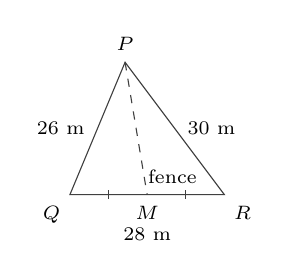
\begin{tikzpicture}[fig,every node/.style={font=\scriptsize}]
\draw[fig] (0,0) -- (1.96,0) -- (0.7,1.68) -- cycle;
\draw[fig,dashed] (0.7,1.68) -- (0.98,0);
\draw[fig] (0.49,-0.055) -- (0.49,0.055);
\draw[fig] (1.47,-0.055) -- (1.47,0.055);
\node[above] at (0.7,1.71) {$P$};
\node[below left] at (0,-0.03) {$Q$};
\node[below right] at (1.96,-0.03) {$R$};
\node[below] at (0.98,-0.03) {$M$};
\node[below] at (0.98,-0.3) {$28$~m};
\node[left] at (0.31,0.84) {$26$~m};
\node[right] at (1.37,0.84) {$30$~m};
\node[right,inner sep=1pt] at (0.95,0.22) {fence};
\end{tikzpicture}
\end{center}}

\expandafter\def\csname fig@c11\endcsname{%
\begin{center}
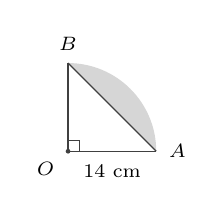
\begin{tikzpicture}[fig,every node/.style={font=\scriptsize}]
\fill[figfill2] (1.12,0) arc (0:90:1.12) -- cycle;
\draw[fig] (0,0) -- (1.12,0);
\draw[fig] (0,0) -- (0,1.12);
\draw[fig] (1.12,0) -- (0,1.12);
\draw[fig] (0.14,0) -- (0.14,0.14) -- (0,0.14);
\fill[figline] (0,0) circle (0.03);
\node[below] at (0.56,-0.05) {$14$~cm};
\node[below left] at (-0.05,-0.02) {$O$};
\node[right] at (1.16,0) {$A$};
\node[above] at (0,1.16) {$B$};
\end{tikzpicture}
\end{center}}

\expandafter\def\csname fig@c12q\endcsname{%
\begin{center}
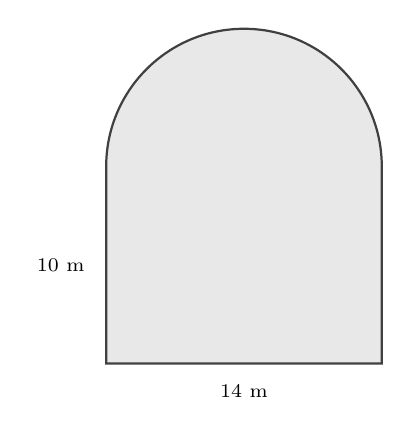
\begin{tikzpicture}[fig,every node/.style={font=\scriptsize}]
\fill[figfill] (-1.75,0) -- (1.75,0) -- (1.75,2.5) arc (0:180:1.75) -- cycle;
\draw[fig,thick] (-1.75,0) -- (1.75,0) -- (1.75,2.5) arc (0:180:1.75) -- cycle;
\node[below] at (0,-0.15) {$14$~m};
\node[left] at (-1.9,1.25) {$10$~m};
\end{tikzpicture}
\end{center}}

\expandafter\def\csname fig@d13\endcsname{%
\begin{center}
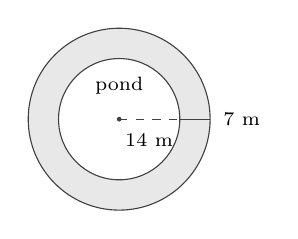
\begin{tikzpicture}[fig,every node/.style={font=\scriptsize}]
\fill[figfill] (0,0) circle (1.155);
\fill[white] (0,0) circle (0.77);
\draw[fig] (0,0) circle (1.155);
\draw[fig] (0,0) circle (0.77);
\draw[fig,dashed] (0,0) -- (0.77,0);
\draw[fig] (0.77,0) -- (1.155,0);
\fill[figline] (0,0) circle (0.03);
\node[below] at (0.38,-0.06) {$14$~m};
\node[right] at (1.2,0) {$7$~m};
\node at (0,0.42) {pond};
\end{tikzpicture}
\end{center}}

\expandafter\def\csname fig@e14q\endcsname{%
\begin{center}
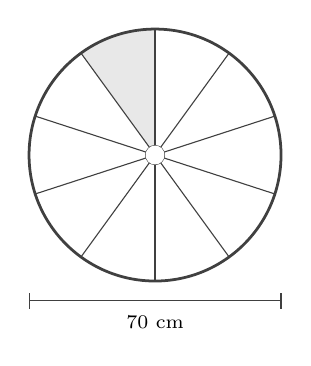
\begin{tikzpicture}[fig,every node/.style={font=\scriptsize}]
\fill[figfill] (0,0) -- (90:1.6) arc (90:126:1.6) -- cycle;
\draw[fig,line width=1pt] (0,0) circle (1.6);
\foreach \a in {18,54,90,126,162,198,234,270,306,342}
  \draw[fig] (\a:0.12) -- (\a:1.6);
\draw[fig] (0,0) circle (0.12);
\fill[white] (0,0) circle (0.12);
\draw[fig] (-1.6,-1.85) -- (1.6,-1.85);
\draw[fig] (-1.6,-1.95) -- (-1.6,-1.75);
\draw[fig] (1.6,-1.95) -- (1.6,-1.75);
\node[below] at (0,-1.92) {$70$~cm};
\end{tikzpicture}
\end{center}}

\expandafter\def\csname fig@e14a\endcsname{%
\begin{center}
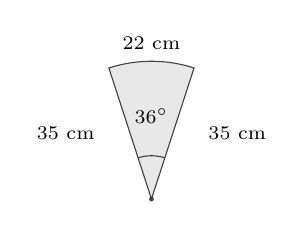
\begin{tikzpicture}[fig,every node/.style={font=\scriptsize}]
\fill[figfill] (0,0) -- (72:1.75) arc (72:108:1.75) -- cycle;
\draw[fig] (0,0) -- (72:1.75) arc (72:108:1.75) -- cycle;
\draw[fig] (72:0.55) arc (72:108:0.55);
\node at (90:1.05) {$36^\circ$};
\node[right] at (0.6,0.83) {$35$~cm};
\node[left] at (-0.6,0.83) {$35$~cm};
\node at (0,1.98) {$22$~cm};
\fill[figline] (0,0) circle (0.03);
\end{tikzpicture}
\end{center}}
\makeatother
